\documentclass[25pt, a0paper, portrait]{tikzposter}
\usetheme{Desert} % A professional, premium theme
\usepackage{booktabs}
\usepackage{tikz}
\usetikzlibrary{arrows.meta, positioning, shapes.geometric, calc}

\title{The Knowledge Lifecycle of Large Language Models}
\author{Amey Thakur}
\institute{Research Presentation, 2026}

\begin{document}

\maketitle

\begin{columns}
    \column{0.5}
    \block{1. The Fragmentation Problem}{
        Current LLM knowledge management is siloed into subfields like RAG, Editing, and Continual Learning. We optimize these in isolation, but fail at the \textbf{boundaries}.
        \begin{itemize}
            \item \textbf{Issue:} No unified formalism for the "life" of a fact.
            \item \textbf{Consequence:} Epistemic desynchronisation and untrustworthy agents.
        \end{itemize}
    }

    \block{2. The Knowledge Lifecycle Framework}{
        \centering
        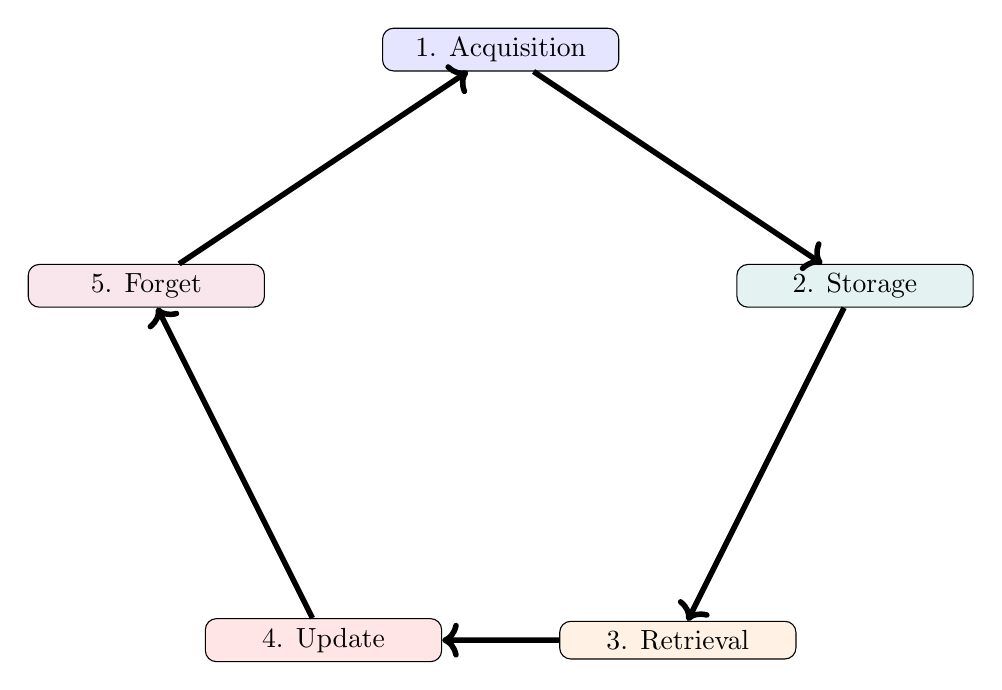
\begin{tikzpicture}[scale=1.5]
            \node[draw, rounded corners, fill=blue!10, minimum width=3cm] (acq) at (0,3) {1. Acquisition};
            \node[draw, rounded corners, fill=teal!10, minimum width=3cm] (sto) at (3,1) {2. Storage};
            \node[draw, rounded corners, fill=orange!10, minimum width=3cm] (ret) at (1.5,-2) {3. Retrieval};
            \node[draw, rounded corners, fill=red!10, minimum width=3cm] (upd) at (-1.5,-2) {4. Update};
            \node[draw, rounded corners, fill=purple!10, minimum width=3cm] (fgt) at (-3,1) {5. Forget};
            
            \draw[->, line width=2pt] (acq) -- (sto);
            \draw[->, line width=2pt] (sto) -- (ret);
            \draw[->, line width=2pt] (ret) -- (upd);
            \draw[->, line width=2pt] (upd) -- (fgt);
            \draw[->, line width=2pt] (fgt) -- (acq);
        \end{tikzpicture}
        \vspace{1cm}
        We define 5 structural stages: Acquisition, Storage, Retrieval, Update, and Forgetting. The interactions between these stages are the source of modern AI failure modes.
    }

    \column{0.5}
    \block{3. Metric: Lifecycle Desynchronisation ($\mathcal{D}_{sync}$)}{
        We introduce a formal cross-modal metric to quantify the conflict between internal memory ($\theta$) and external context ($\mathcal{M}$).
        \begin{equation*}
            \mathcal{D}_{sync} = D_{KL}(P(y|q, \theta_{now}, \mathcal{M}_{now}) \| P(y|q, \theta_{stale}, \mathcal{M}_{now}))
        \end{equation*}
        $\mathcal{D}_{sync} > 1.0$ indicates a system that is no longer epistemically consistent.
    }

    \block{4. Intervention: The Provenance Vector ($p$)}{
        \begin{itemize}
            \item \textbf{Mechanism:} Appending temporal metadata $[\tau_i; s_i]$ to every stored fact in the FFN.
            \item \textbf{Activation Steering:} Dynamically "muting" old facts during test-time compute.
        \end{itemize}
        \centering
        \begin{equation*}
            S(\Delta \tau_i) = \sigma(\beta \cdot \Delta \tau_i - \gamma)
        \end{equation*}
        Provenance steering resolves conflicts without retraining.
    }

    \block{5. Case Study: Vioxx Withdrawal}{
        We simulated the 2004 Vioxx medical withdrawal across modalities.
        \begin{itemize}
            \item \textbf{Unsynced System:} Ignores withdrawal labels; recommends dangerous drug.
            \item \textbf{Synced System ($\mathcal{D}_{sync} \to 0$):} Correctly resolves conflict using Provenance Steering.
        \end{itemize}
        Validated on GPT-2 and LLaVA-1.5 architectures.
    }

    \block{6. Conclusion}{
        Maintaining epistemic consistency is the next frontier of AI safety. The Knowledge Lifecycle framework provides the roadmap for reliable, time-aware autonomous agents.
    }
\end{columns}

\end{document}
